%\documentclass[10pt,spanish,a4paper,openany,notitlepage]{article}
\documentclass[a4paper,10pt]{article}

%-------------------------------------Paquetes-----------------------------------------------------------------------
\usepackage[spanish]{babel}  	% Traduce los textos a castellano
\usepackage[utf8]{inputenc}	% Permite escribir directamente áéíóúñ
\usepackage{t1enc}            	% Agrega caracteres extendidos al font
\usepackage{amsmath} 		%Permite imprimir mas opcciones matematicas
\usepackage{graphicx}		%Permite agregar imagenes al informe
\usepackage{multicol}  		%Permite dividir el texto en varias columnas
\usepackage{anysize}		%Permite modificar los margenes del documento
\usepackage{float} 		%Permite utilizar H para colocar las imagenes en un lugar especifico 

% Paquete para dividir las tablas en subtablas
\usepackage{multirow}

%estos 2 sirven para achicar la tabla
\usepackage{booktabs}
\usepackage{tabulary}

\usepackage[spanish]{babel}
%------------------------------------------------------------------------------------------------------------------------

%---------------------------------------Configuraciones de pagina-------------------------------------------------
\marginsize{2.5cm}{2.5cm}{1cm}{1cm}
%------------------------------------------------------------------------------------------------------------------------
%---------------------------------------Definiciones propias---------------------------------------------------------
\newcommand{\grad}{\hspace{-2mm}$\phantom{a}^{\circ}$} %El º que no existe como comando
\newcommand{\oiint}{\displaystyle\bigcirc\!\!\!\!\!\!\!\!\int\!\!\!\!\!\int} %Integral doble cerrada
%------------------------------------------------------------------------------------------------------------------------

\author{
  Funes, Pablo N \\ 94894 \\
  \texttt{funestunes@hotmail.com}
  \and
 Vazquez, Matias F \\ 91523\\
  \texttt{mfvazquez@gmail.com}
  \and
 Luizaga, Ricardo \\ 87528\\
  \texttt{riluizaga@gmail.com}
}
\title{TP N\grad 3: Dispositivos de potencia}

\date{}

\begin{document}

\maketitle
	\title \author



\section{Objetivos del trabajo} %El * se usa para evitar numerar las secciones
Afianzar los conocimientos teóricos respecto de los dispositivos de potencia. Analizar la conplejidad que pueden llegar a tener los circuitos asociados al disparo de dispositivos de potencia. Para ello, se trabajará con circuitos prestablecidos.

\section{IGBT}

\subsection{Analisis preliminar}

\begin{figure}[H] %[h] para here [b] para bottom [t] para top [H]+float para aqui si o si
\begin{center}
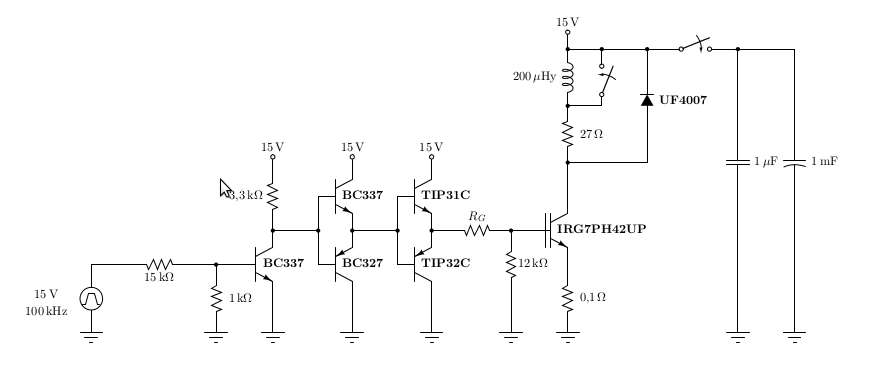
\includegraphics[scale=0.5]{./imagenes/Circuito_IGBT.png}
\caption{Circuito simplificado de disparo de un IGBT.}
 \label{fig:Circuito_IGBT}
\end{center}
\end{figure}

\begin{enumerate}
	\item[•] Explicar por qué los transistores ocupan el lugar que ocupan, es decir, por qué es necesario que cada etapa tenga la capacidad de manejar cada vez mas corriente.
	\item[•]	 Identificar qué función cumple R$_ {G}$ en el circuito. ¿Que sucede si R$_ {G}$ = 18$\Omega$ o R$_ {G}$ = 1k$\Omega$? Estime la corriente que puede circular por la misma, y calcule en forma aproximada el tiempo que tarda la tensión de Gate del IGBT en establecerse.
	\item[•] ¿Que función cumple el diodo UF4007?
\end{enumerate}

\subsection{Mediciones del circuito}

\subsubsection{Caida de tensión y corriente en el resistor R$_ {G}$}

\subsubsection{Capacidad de entrada}

\subsubsection{Con el inductor cortocircuitado y los capacitores de salida conectados}

\subsubsection*{Corriente que circula por el IGBT durante las transiciones}
\subsubsection*{Energia consumida durante cada transicion}
\subsubsection*{Potencia disipada}

\subsubsection{Con el inductor conectado y los capacitores de salida conectados}

\subsubsection*{Corriente que circula por el IGBT durante las transiciones}
\subsubsection*{Energia consumida durante cada transicion}
\subsubsection*{Potencia disipada}

\subsubsection{Con el inductor conectado y los capacitores de salida desconectados}

\subsubsection*{Corriente que circula por el IGBT durante las transiciones}
\subsubsection*{Energia consumida durante cada transicion}
\subsubsection*{Potencia disipada}

\subsection{Análisis de mediciones}

\begin{enumerate}
	\item[•] ¿Por que es necesario entregar mucha corriente al gate del IGBT?¿Que importancia tiene la resistencia serie del circuito que se encarga de controlar el Gate de este dispositivo?
	
	\item[•]	 ¿Que ocurre si se desea controlar al IGBT con una salida digital típica de un microcontrolador, donde la máxima corriente que se puede entregar es de algunos pocos miliAmperes?
	
	\item[•] A partir de la estimación de potencia disipada y de los datos térmicos de las hojas de datos realizar el analisis térmico del IGBT y calcular la temperatura de juntura.
	
	\item[•] ¿Por qué varía la corriente del IGBT con y sin el inductor conectado?
	
\end{enumerate}

\section{Tiristores}

\subsection{Analisis preliminar}

\begin{figure}[H] %[h] para here [b] para bottom [t] para top [H]+float para aqui si o si
\begin{center}
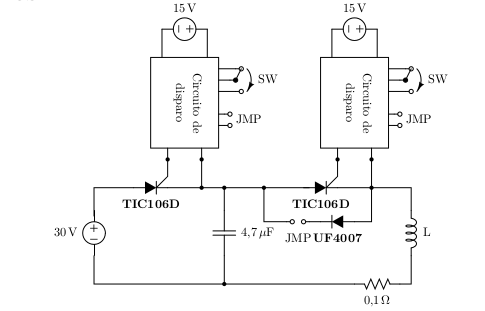
\includegraphics[scale=0.5]{./imagenes/Circuito_Tiristores.png}
\caption{Circuito esquemático simplificado de disparo de dos Tiristores. }
 \label{fig:Circuito_tiristores}
\end{center}
\end{figure}

\subsection{Mediciones del circuito}

\subsubsection{Diodo desconectado y disparo corto}

\subsubsection*{Tensión en el inductor respecto del terminal negativo de la fuente}
\subsubsection*{Corriente}
\subsubsection*{Tensión en el resistor}

\subsubsection{Diodo conectado y disparo corto}

\subsubsection*{Tensión en el inductor respecto del terminal negativo de la fuente}
\subsubsection*{Corriente}
\subsubsection*{Tensión en el resistor}

\subsubsection{Diodo conectado y disparo largo}

\subsubsection*{Tensión en el inductor respecto del terminal negativo de la fuente}
\subsubsection*{Corriente}
\subsubsection*{Tensión en el resistor}

\section{Análisis de las mediciones}

\begin{enumerate}
	\item[•] Por qué se producen distintas formas de onda para cada una de las configuraciones medidas.
	
	\item[•]	 Por qué para cargar el capacitor de 4,7$\mu$F alcanza para realizar un disparo corto.
	
\end{enumerate}

\section{Conclusión}

\end{document}